\documentclass{article}
\usepackage{graphicx} % Required for inserting images
\usepackage{amsmath}
\title{Práctica 1}
\author{Adam Bourbahh Romero}
\date{28/09/2025}

\begin{document}

\maketitle
\section{Análisis teórico del algoritmo Merge sort}
Para este apartado he elegido la ordenación por mezcla. Este algoritmo recursivo consiste en la "división" recursiva de, por ejemplo, un array. Imaginemos que tenemos un array de 4 elementos \textbf{[3,1,5,8]} y queremos darle un orden ascendente.
\subsection{División}
Nuestro algoritmo lo que hace en este caso es dividir el array a la mitad de forma constante hasta tener cada elemento separado. Podemos intuir a partir de esto que el algoritmo va a hacer $\textbf{log}_2\textbf{(n)}$ divisiones.

Con el ejemplo dado, nuestro algoritmo convierte \textbf{[3,1,5,8]} $\xrightarrow{\text{1}}$ \textbf{[3,1]} + \textbf{[5,8]} $\xrightarrow{\text{2}}$ \textbf{[3]}+\textbf{[1]} \textbf{[5]}+\textbf{[8]}. Podríamos pensar que en este proceso se hacen 3 operaciones, sin embargo aquí medimos el número de "niveles recursivos".

\includegraphics[scale=0.2]{Screenshot_20250923_105754_Samsung Notes.jpg}

En el árbol que he adjuntado podemos ver como solo hay 2 niveles antes de llegar a las hojas del árbol.

\newpage
\subsection{Mezcla}

La siguiente gran parte de este algoritmo consiste en ir de forma "ascendente" por el árbol para reordenar los subarrays, dado que en total hay n elementos, vemos fácilmente que se ejecutará en tiempo lineal.

\includegraphics[scale=0.2]{Screenshot_20250923_111651_Samsung Notes.jpg}

\subsection{Total}
Al principio he adelantado que la complejidad del algoritmo es de \textbf{O(n*log n)}. 
Sin embargo podríamos pensar que por qué no es directamente O(n). Para clarificar esto, volvamos al esquema de árbol. Hemos dicho que teníamos log(n) niveles. Además, en cada uno de esos niveles se hacen n operaciones. Por ejemplo, en el último nivel de nuestro ejemplo se hacen una por cada rama, es decir, $1x4=4$ y en el segundo nivel, hacemos dos operaciones por cada rama, es decir, $2x2=4$.
Por tanto, tenemos n operaciones en cada nivel : \[\underbrace{$n + n + \dots + n$}_{log(n) \text{veces}} \]
Equivalentemente, $\mathbf{nlog(n)}$ \textbf{operaciones.}

\newpage
\section{Cálculo de la eficiencia empírica}
Una vez realizado el cálculo de teórico, vamos a ver que tanto se acerca a la eficiencia empírica.
Habiendo ejecutado el código con distintos tamaños:
\begin{center}
\begin{tabular}{|p{4cm}|p{4cm}|}
    \hline
    Nº Datos & T. Ejecución \\
    \hline
    100 & 4.918e-06 \\
    \hline
    500 & 2.5652e-05 \\
    \hline
    1000 & 5.3912e-05 \\
    \hline
    5000 & 0.000389048 \\
    \hline
    6000 & 0.000508194 \\
    \hline
    8000 & 0.000627804 \\
    \hline
    10000 & 0.000849083 \\
    \hline
    12000 & 0.006077 \\
    \hline
\end{tabular}

A la hora de graficarlo podemos ver que el tiempo de ejecución se asemeja mucho a $\mathbf{f(x)=xlog(x)}$ :
 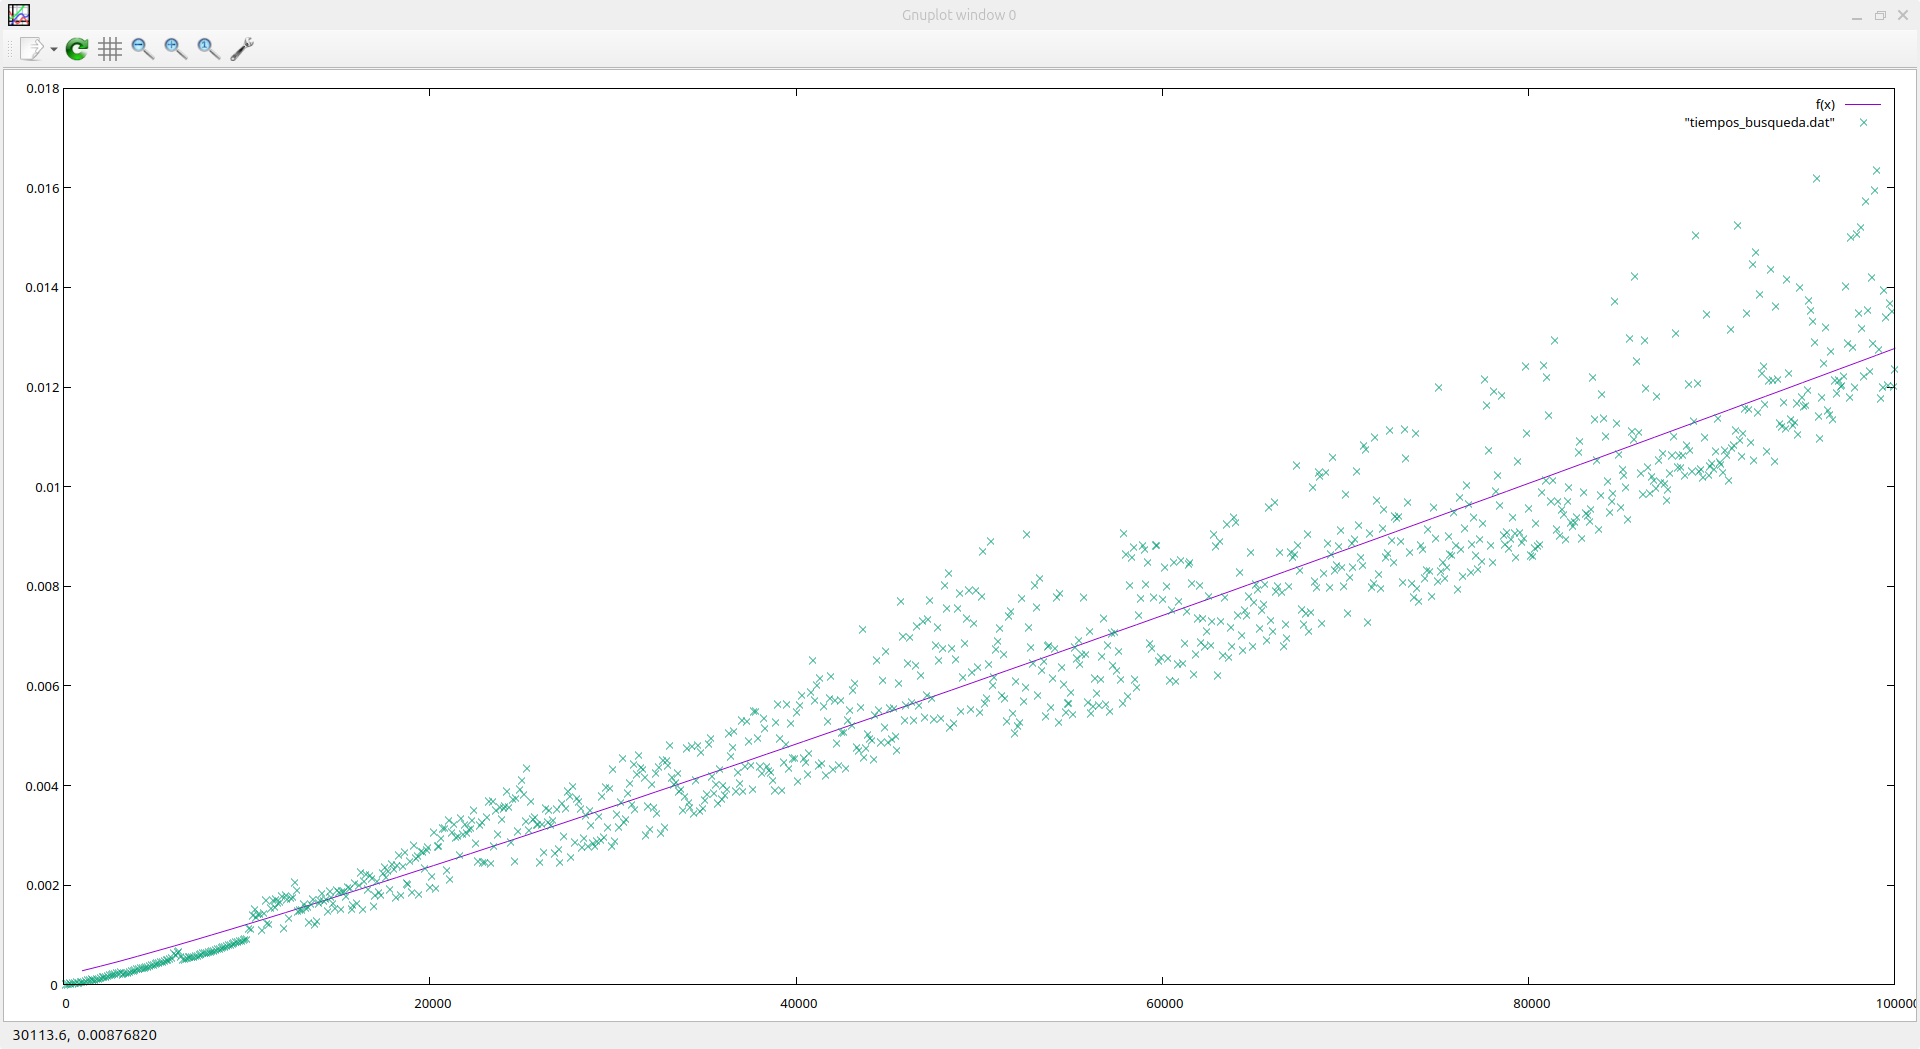
\includegraphics[scale=0.5]{plot.png}
    \end{center}

Sin embargo, la muestra de datos no es suficiente como para poder asegurarlo, por lo que usando el csh que se nos ha dado, lo he modificado para que funcione con el mergesort y he generado un archivo con cientos de ejecuciones. Tras ello, he usado la herramiento \textbf{fit} de gnuplot para averiguar el a y b que se adecue a $a*x*log(x)+b$. Por último, he hecho un plot de ambas gráficas y podemos ver un comportamiento claramente parecido. Adjunto a continuación las capturas:

\includegraphics[scale=0.5]{Captura desde 2025-09-28 18-23-13.png}

\includegraphics[scale=0.2]{Captura desde 2025-09-28 18-23-29.png}


\end{document}